\documentclass[11pt, a4paper, twocolumn]{article}

% --- UNIVERSAL PREAMBLE BLOCK ---
\usepackage[a4paper, top=2.5cm, bottom=2.5cm, left=2cm, right=2cm]{geometry}
\usepackage{fontspec}

\usepackage[english, bidi=basic, provide=*]{babel}

\babelprovide[import, onchar=ids fonts]{english}

% Set default/Latin font to Sans Serif in the main (rm) slot
\babelfont{rm}{Noto Sans}

% --- REQUIRED PACKAGES ---
\usepackage{amsmath}
\usepackage{booktabs}
\usepackage{graphicx}
\usepackage{hyperref} % Must be the last package loaded

% --- TEMPLATE COMPATIBILITY MACROS ---
% These macros allow the iLCSS custom template tags to compile natively 
% in a standard LaTeX environment without requiring the external ilcss.cls file.
\usepackage{authblk}
\newcommand{\templatetype}[1]{}
\newcommand{\leadauthor}[1]{}

\newcommand{\storedsig}{}
\newcommand{\significancestatement}[1]{\renewcommand{\storedsig}{\vspace{1em}\noindent\textbf{Significance Statement: } #1 \par\vspace{1em}}}

\newcommand{\authorcontributions}[1]{}
\newcommand{\authordeclaration}[1]{}
\newcommand{\equalauthors}[1]{}

\newcommand{\storedcorr}{}
\newcommand{\correspondingauthor}[1]{\renewcommand{\storedcorr}{\vspace{1em}\noindent\textit{#1}\par}}

\newcommand{\storedkeys}{}
\newcommand{\keywords}[1]{\renewcommand{\storedkeys}{\noindent\textbf{Keywords: } #1 \par\vspace{1em}}}

\newcommand{\storeddates}{}
\newcommand{\dates}[1]{\renewcommand{\storeddates}{\vspace{1em}\noindent\textit{#1}\par}}

\newcommand{\doi}[1]{}
\newcommand{\dropcap}[1]{\noindent\textbf{\Large #1}}
\newcommand{\acknow}[1]{\section*{Acknowledgments} #1}
\newcommand{\showacknow}{}

\let\oldmaketitle\maketitle
\renewcommand{\maketitle}{%
  \oldmaketitle
  \storedsig
  \storedcorr
  \storedkeys
  \storeddates
}

% --- DOCUMENT METADATA ---
\templatetype{ilcssworkingpaper}

\title{Extending Deterministic Population Projections:\\ \large A Scenario-Based Hamilton-Perry Approach for Kota Semarang (2035--2050)}

% Use letters for affiliations, numbers to show equal authorship (if applicable) and to indicate the corresponding author
\author[1,2*]{Ricardo Ochoa}
\author[1]{Socorro Román}

\affil[1]{CAPSUS}

\leadauthor{ricardo.ochoa@capsus.mx}

\significancestatement{Demographic projections for sub-national regions are often constrained by the lack of granular vital statistics. This paper presents a methodological framework to extend official deterministic projections using the macroscopic Hamilton-Perry method. Applied to Kota Semarang, Indonesia, this approach demonstrates how historical cohort change ratios and child-to-woman ratios can be used to generate robust scenario-based forecasts (Minimum, Mean, Maximum) through 2050. This provides critical insights for urban planning and policy formulation, mitigating the risk of ecological fallacy inherent in applying national-level models to local urban contexts.}

\authorcontributions{R.O. developed the conceptual framework and executed the data analysis. S.R. provided methodological revisions and benchmark validation.}
\authordeclaration{The authors declare no conflict of interest.}
\correspondingauthor{\textsuperscript{2} E-mail: ricardo.ochoa@capsus.mx}

\keywords{Demography $|$ Hamilton-Perry Method $|$ Population Projections $|$ Urban Planning $|$ Kota Semarang}

\dates{This manuscript was compiled on \today}

\doi{\url{http://ilcss.umd.edu/}}

\begin{document}

\maketitle

\begin{abstract}
Standard demographic forecasting relies heavily on the Cohort-Component Method (CCM), requiring highly granular vital rates. At sub-national levels, such as specific municipalities, these granular arrays are often unavailable, limiting projections to deterministic outputs from central statistical agencies. This paper outlines an extension of the official 2020--2035 projections for Kota Semarang, Central Java, utilizing the Hamilton-Perry method. By treating survivorship and migration as combined empirical ratios based on historical age-sex structures, we mathematically project the population to 2050. To address the uncertainty inherent in deterministic baselines, three bounding scenarios (Minimum, Mean, Maximum) are constructed using observed variations in Cohort Change Ratios (CCRs) and Child-Woman Ratios (CWRs). The resulting projections are benchmarked against national-level United Nations World Population Prospects, confirming the macro-demographic validity of the local trajectory. This framework provides a reproducible model for extending limited local demographic data into robust, long-term scenario forecasts.
\end{abstract}

\dropcap{D}emographic projections constitute the essential scaffolding for long-term urban planning, infrastructure development, and socioeconomic policy formulation. While national projections benefit from robust civil registration and comprehensive demographic surveys, local and municipal planning frequently encounters severe data constraints. This paper outlines the methodology used to extend the population projections for Kota Semarang, Central Java, from 2035 to 2050 while accounting for these specific constraints.

The baseline data used for this extension are the official 2020--2035 projections published by Statistics Indonesia (Badan Pusat Statistik - BPS), derived from the 2020 Population Census (SP2020) \cite{bps2020}. The primary objective of this model is to generate a robust mathematical extension of the BPS data while preserving the complex demographic assumptions embedded in the original official figures, ultimately generating a plausible scenario range (Minimum, Mean, Maximum) for the year 2050.

\section*{Methodological Rationale and Data Constraints}

Standard demographic forecasting predominantly uses the Cohort-Component Method (CCM), which projects the population by modeling births, deaths, and migration as separate, independent components. Executing a traditional CCM from scratch necessitates highly granular, localized data arrays, specifically: Age-Specific Fertility Rates (ASFR), local Age-Specific Mortality Rates (often modeled via Life Tables), and Age-Specific Net Migration Rates (ASNMR).

While BPS uses a deterministic CCM to generate its official projections, it typically publishes only the resulting age-sex population structures and summary indicators (e.g., Total Fertility Rate limits and Life Expectancy targets). The granular age-specific arrays for individual regencies or cities remain unpublished. Furthermore, attempting to bridge this data gap by applying national-level models---such as the United Nations World Population Prospects \cite{un2024}---directly to a specific, highly urbanized metropolitan area like Kota Semarang would result in an \textit{ecological fallacy}, incorrectly assuming local municipal trends mirror national aggregate averages.

To overcome these structural constraints, this projection employs the Hamilton-Perry Method.

\section*{The Hamilton-Perry Method}

The Hamilton-Perry method is a widely recognized macroscopic variant of the Cohort-Component Method. It is explicitly designed for scenarios in which historical age-sex counts are available across consecutive intervals, but detailed vital rates are not. Instead of treating mortality and migration as separate, parameterized inputs, the Hamilton-Perry method combines them into empirical ratios reflecting how specific cohorts move through time. By analyzing the BPS population structures over 5-year intervals (2020 to 2035), the method captures the ``demographic DNA'' of the local population.

The model relies on two primary mathematical mechanisms:

\subsection*{Cohort Change Ratios (CCRs)}
To project the population aged 5 and older, the model calculates Cohort Change Ratios. A CCR measures the combined survivorship and net migration of a specific age cohort over a 5-year period. The standard calculation is given by:

\begin{equation}
    CCR_{x, t} = \frac{P_{x+5, t+5}}{P_{x, t}}
    \label{eq:ccr}
\end{equation}

Where $P$ denotes the population, $x$ is the cohort's starting age, and $t$ is the base year. Because the final demographic age bracket is open-ended (e.g., 75+), its calculation must account for individuals aging into the bracket as well as those already surviving within it:

\begin{equation}
    CCR_{x+, t} = \frac{P_{x+, t+5}}{P_{x-5, t} + P_{x+, t}}
    \label{eq:ccr_open}
\end{equation}

\subsection*{Child-Woman Ratios (CWRs)}
Because children aged 0--4 in the target year ($t+5$) were not yet born in the base year ($t$), CCRs cannot be used to project them. Instead, the model uses a Child-Woman Ratio as an empirical proxy for fertility. The ratio relates the projected number of young children to the projected number of reproductive-age women:

\begin{equation}
    CWR_{t+5} = \frac{P_{0-4, t+5}}{\sum_{x=15}^{49} P_{x, t+5}^{f}}
    \label{eq:cwr}
\end{equation}

Where $P^{f}$ represents the female population. 

\begin{figure}[htbp]
  \centering
	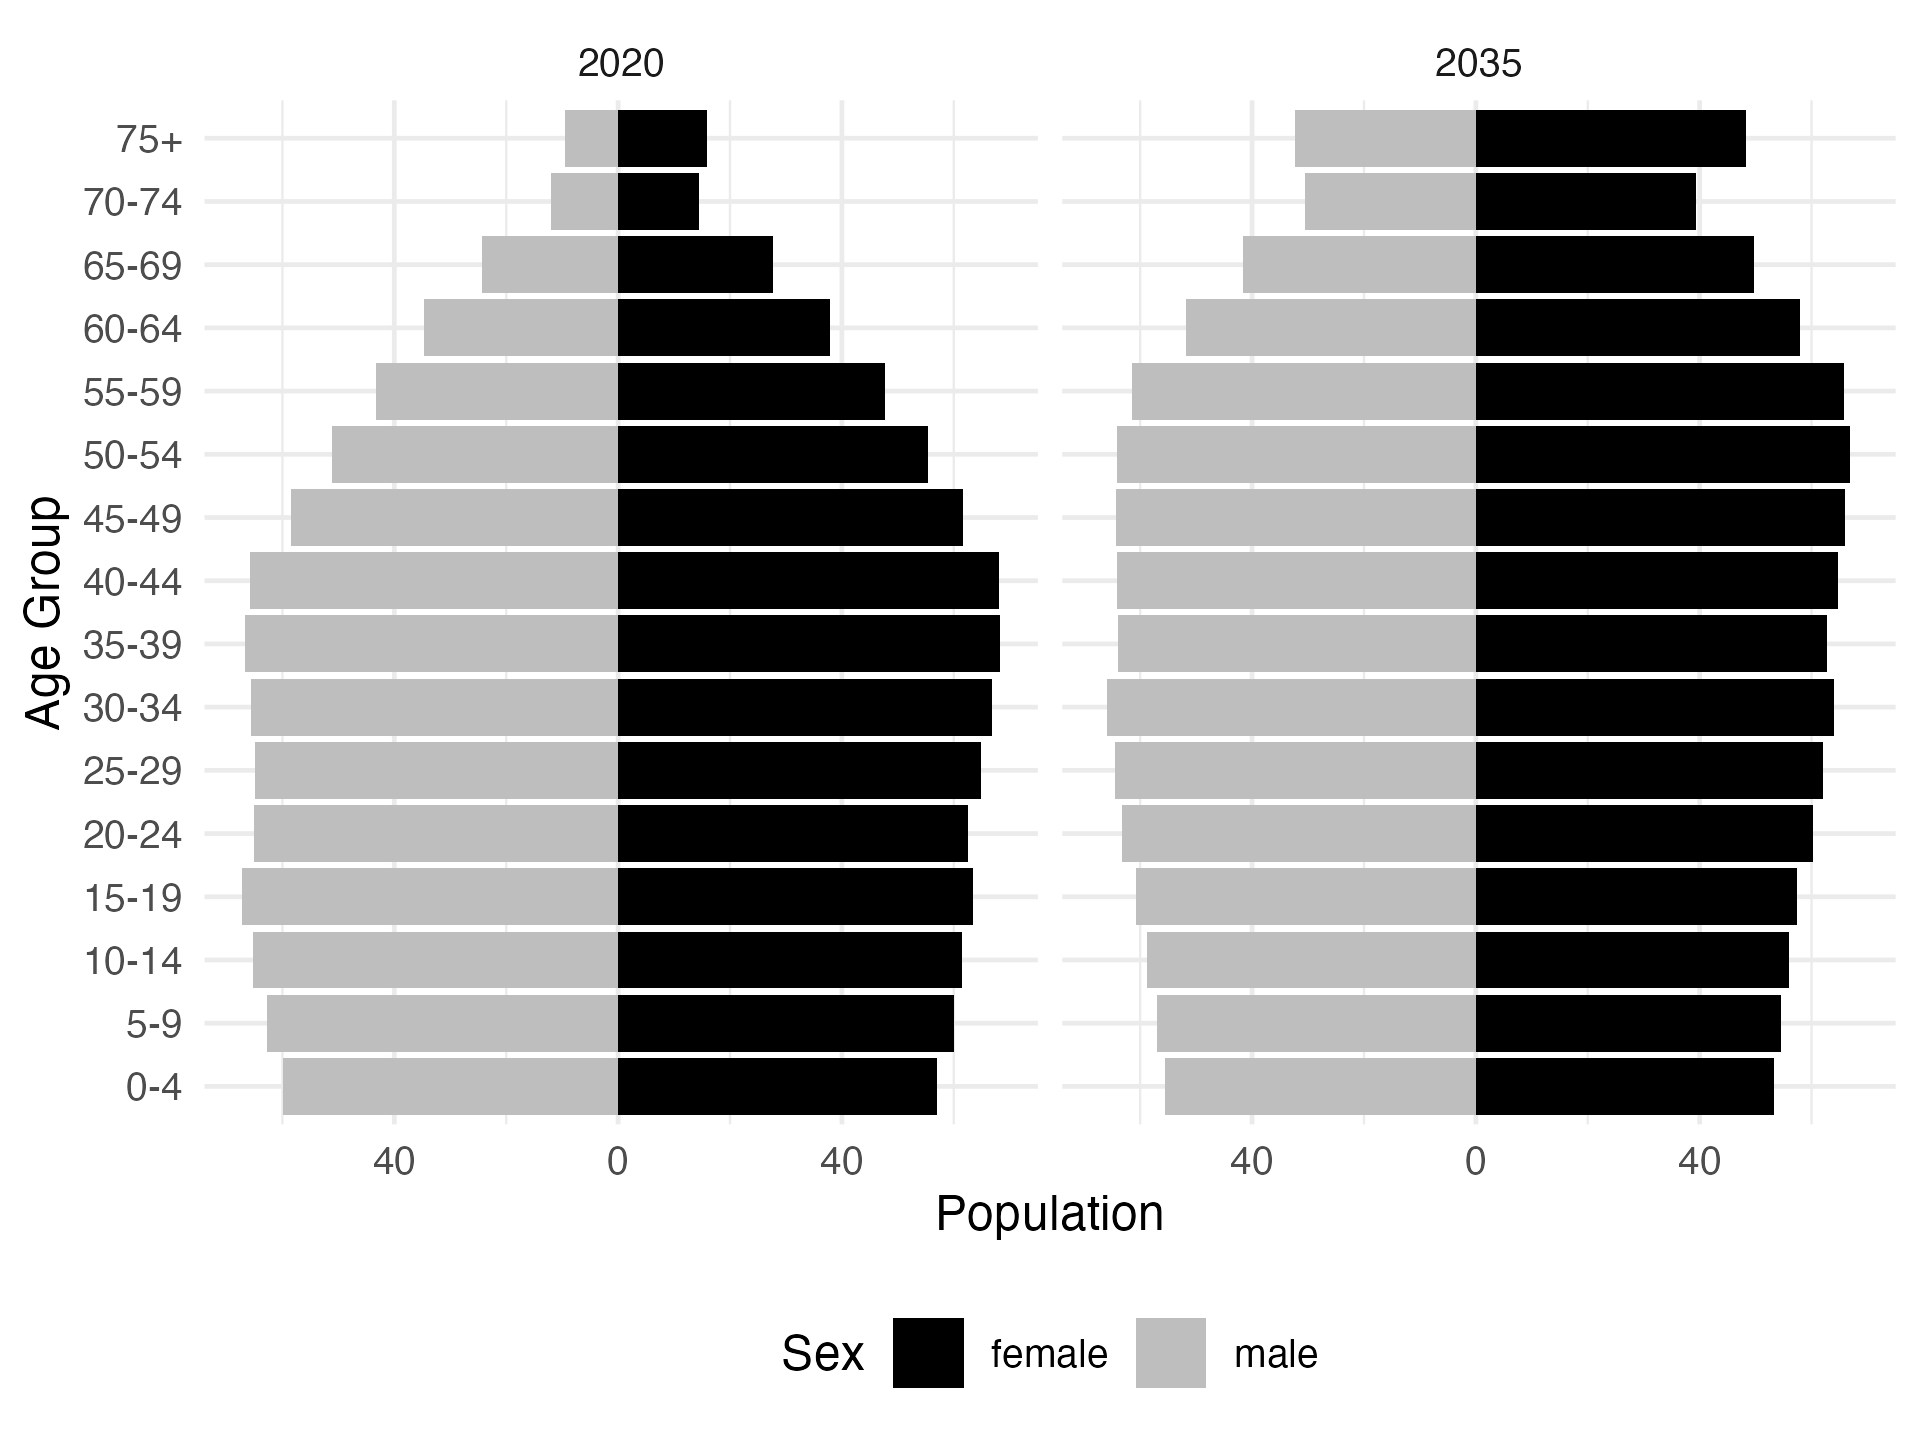
\includegraphics[width=0.5\textwidth]{img/pyramids_bw.png}
  \caption{Comparison of the original official BPS demographic structures from 2020 and 2035, illustrating the baseline population dynamics utilized for CCR extraction.}
  \label{fig:pyramid}
\end{figure}

\section*{Scenario Generation and Uncertainty}

A core limitation of the original BPS projection is its deterministic nature, which yields only a single-point estimate. To address inherent demographic uncertainty, we introduced a scenario-based forecasting approach.

Within the 2020--2035 BPS data, three distinct historical transition periods exist: 2020--2025, 2025--2030, and 2030--2035. The model calculates the CCRs and CWRs for every age-sex cohort across all three periods. From this variance, three bounded parameters are extracted:

\begin{itemize}
    \item \textbf{Minimum Scenario (Low Bound):} Applies the lowest observed ratios, simulating conditions of slower growth, lower fertility, and/or higher out-migration.
    \item \textbf{Mean Scenario (Medium Bound):} Applies the mathematical average of the observed ratios, assuming the baseline trajectory continues steadily.
    \item \textbf{Maximum Scenario (High Bound):} Applies the highest observed ratios, simulating conditions of faster growth, higher fertility, and/or higher in-migration.
\end{itemize}

It is critical to note that BPS explicitly factored macroeconomic variables, such as the relocation of the national capital (Ibu Kota Nusantara - IKN), into their 2020--2035 migration models. By deriving empirical CCRs directly from the BPS data, the Hamilton-Perry model implicitly captures and carries these sophisticated migration assumptions forward into the 2050 forecasts.

\begin{figure}[htbp]
  \centering
	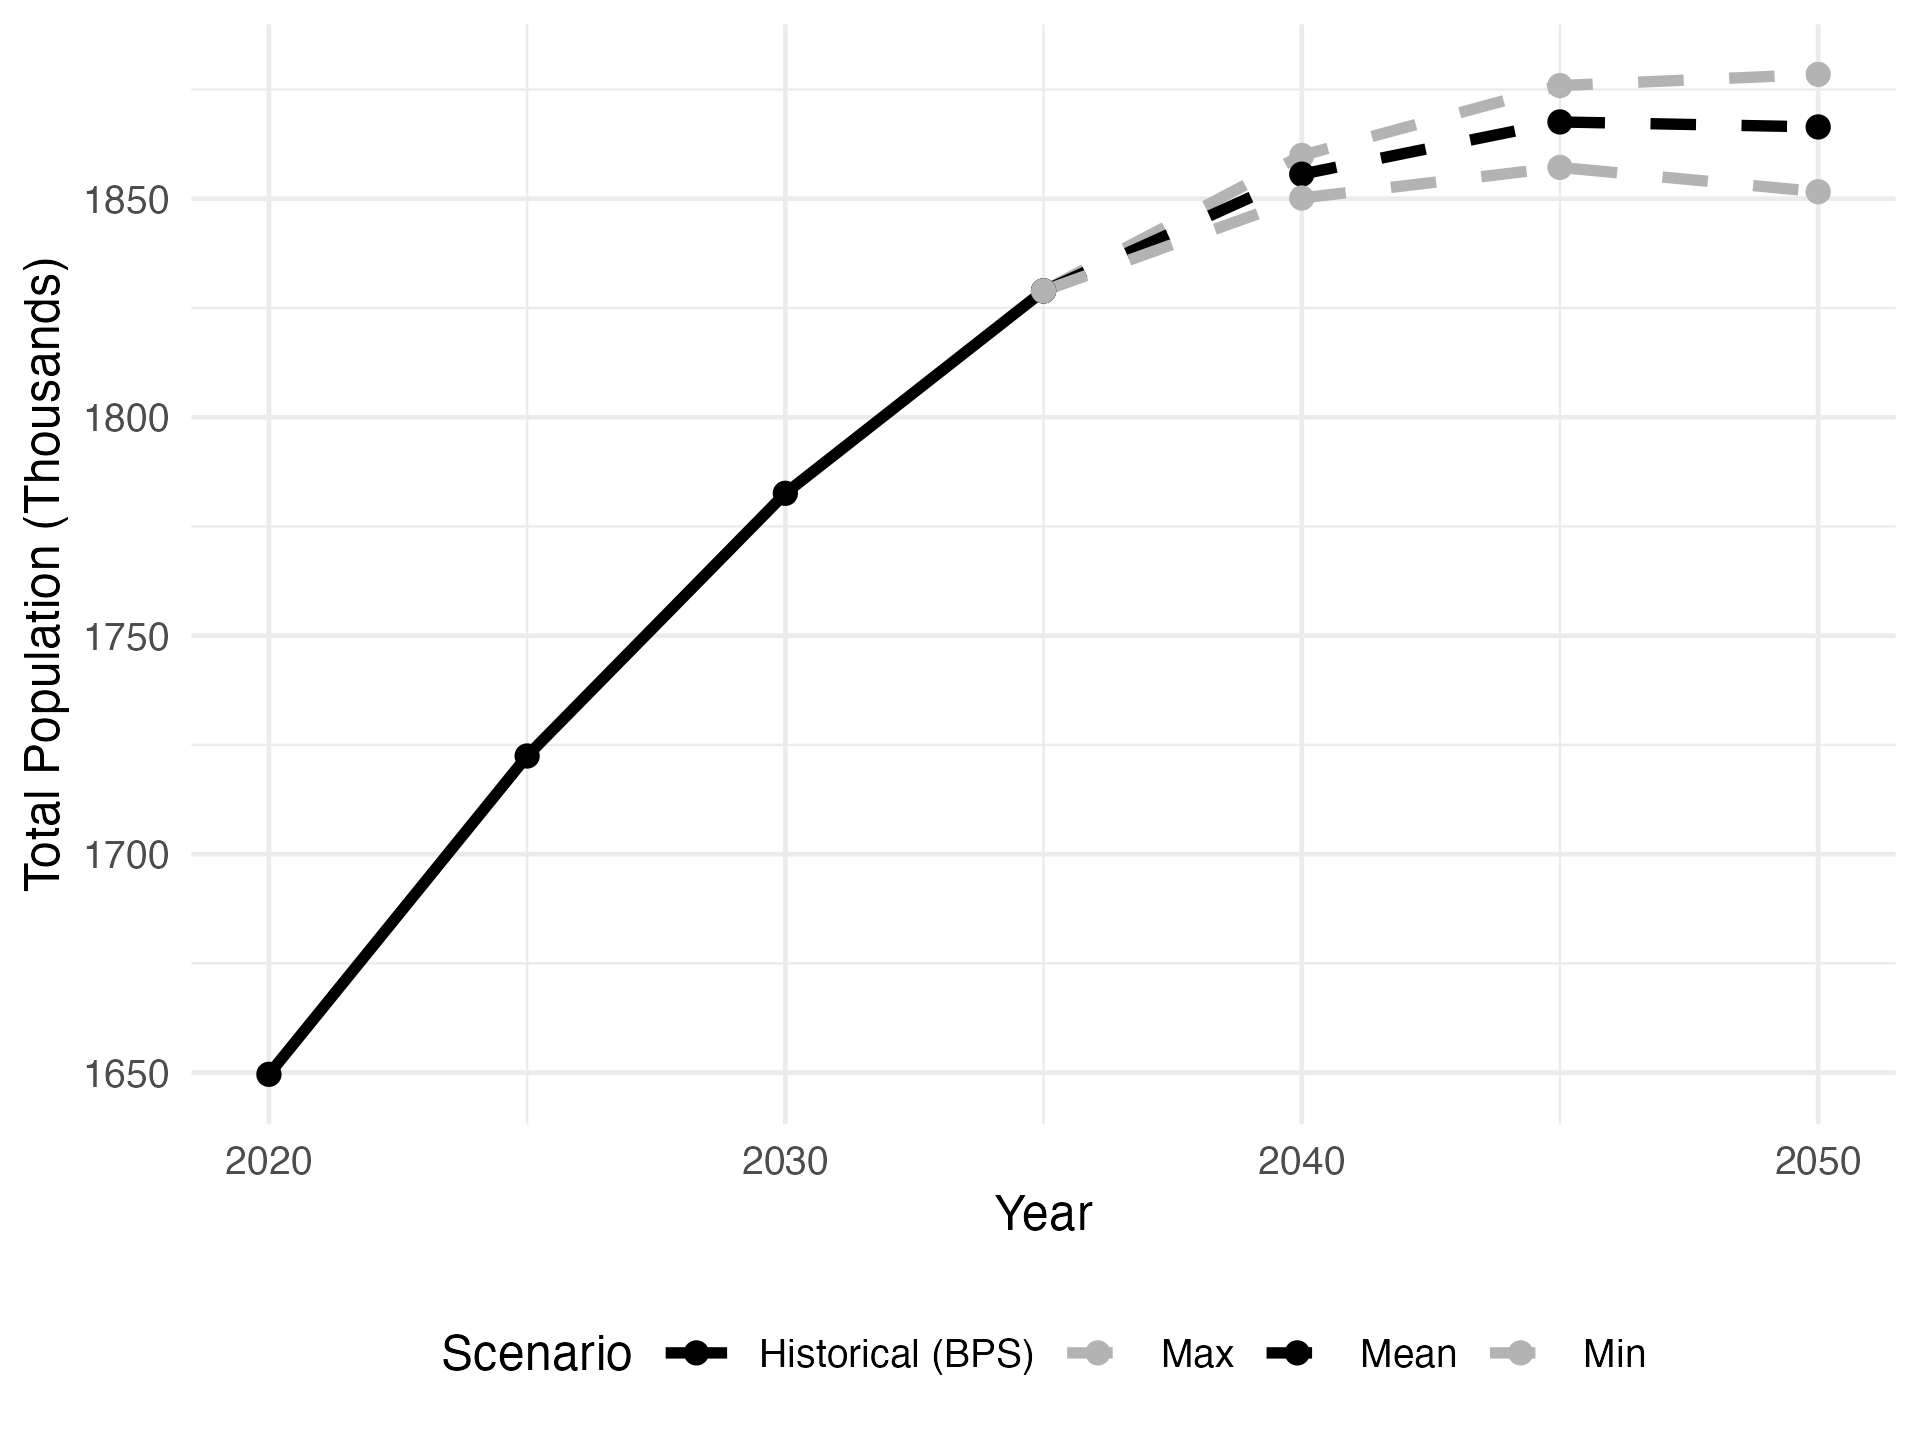
\includegraphics[width=0.5\textwidth]{img/trajectory_bw.png}
  \caption{Total population trajectory showing the historical BPS data seamlessly splitting into the three projected Hamilton-Perry scenarios (Min, Mean, Max) moving toward 2050.}
  \label{fig:trajectory}
\end{figure}


\section*{Step-by-Step Computational Process}

The projection is executed recursively in 5-year iterative steps using a custom computational script in R. For each scenario, the algorithm proceeds as follows:

\begin{enumerate}
    \item \textbf{Establish Base Year:} The model initializes using the final available BPS data point (2035) as the definitive baseline.
    \item \textbf{Project Ages 5+:} The scenario-specific CCRs are multiplied against the 2035 base population to calculate the population aged 5 and older for the year 2040.
    \item \textbf{Calculate Reproductive Base:} The projected 2040 female population aged 15--49 is aggregated.
    \item \textbf{Project Newborns (0--4):} The scenario-specific CWRs are multiplied against the newly calculated 2040 reproductive base to generate the 0--4 age group.
    \item \textbf{Recursive Iteration:} The completed 2040 population structure becomes the new base year. The process is repeated to project 2045, and subsequently 2050.
\end{enumerate}

\section*{External Validation}

While national-level data cannot be mathematically integrated into the local model without causing ecological distortion, the resulting scenario projections must still pass macro-demographic validity checks. 

\begin{figure}[htbp]
  \centering
	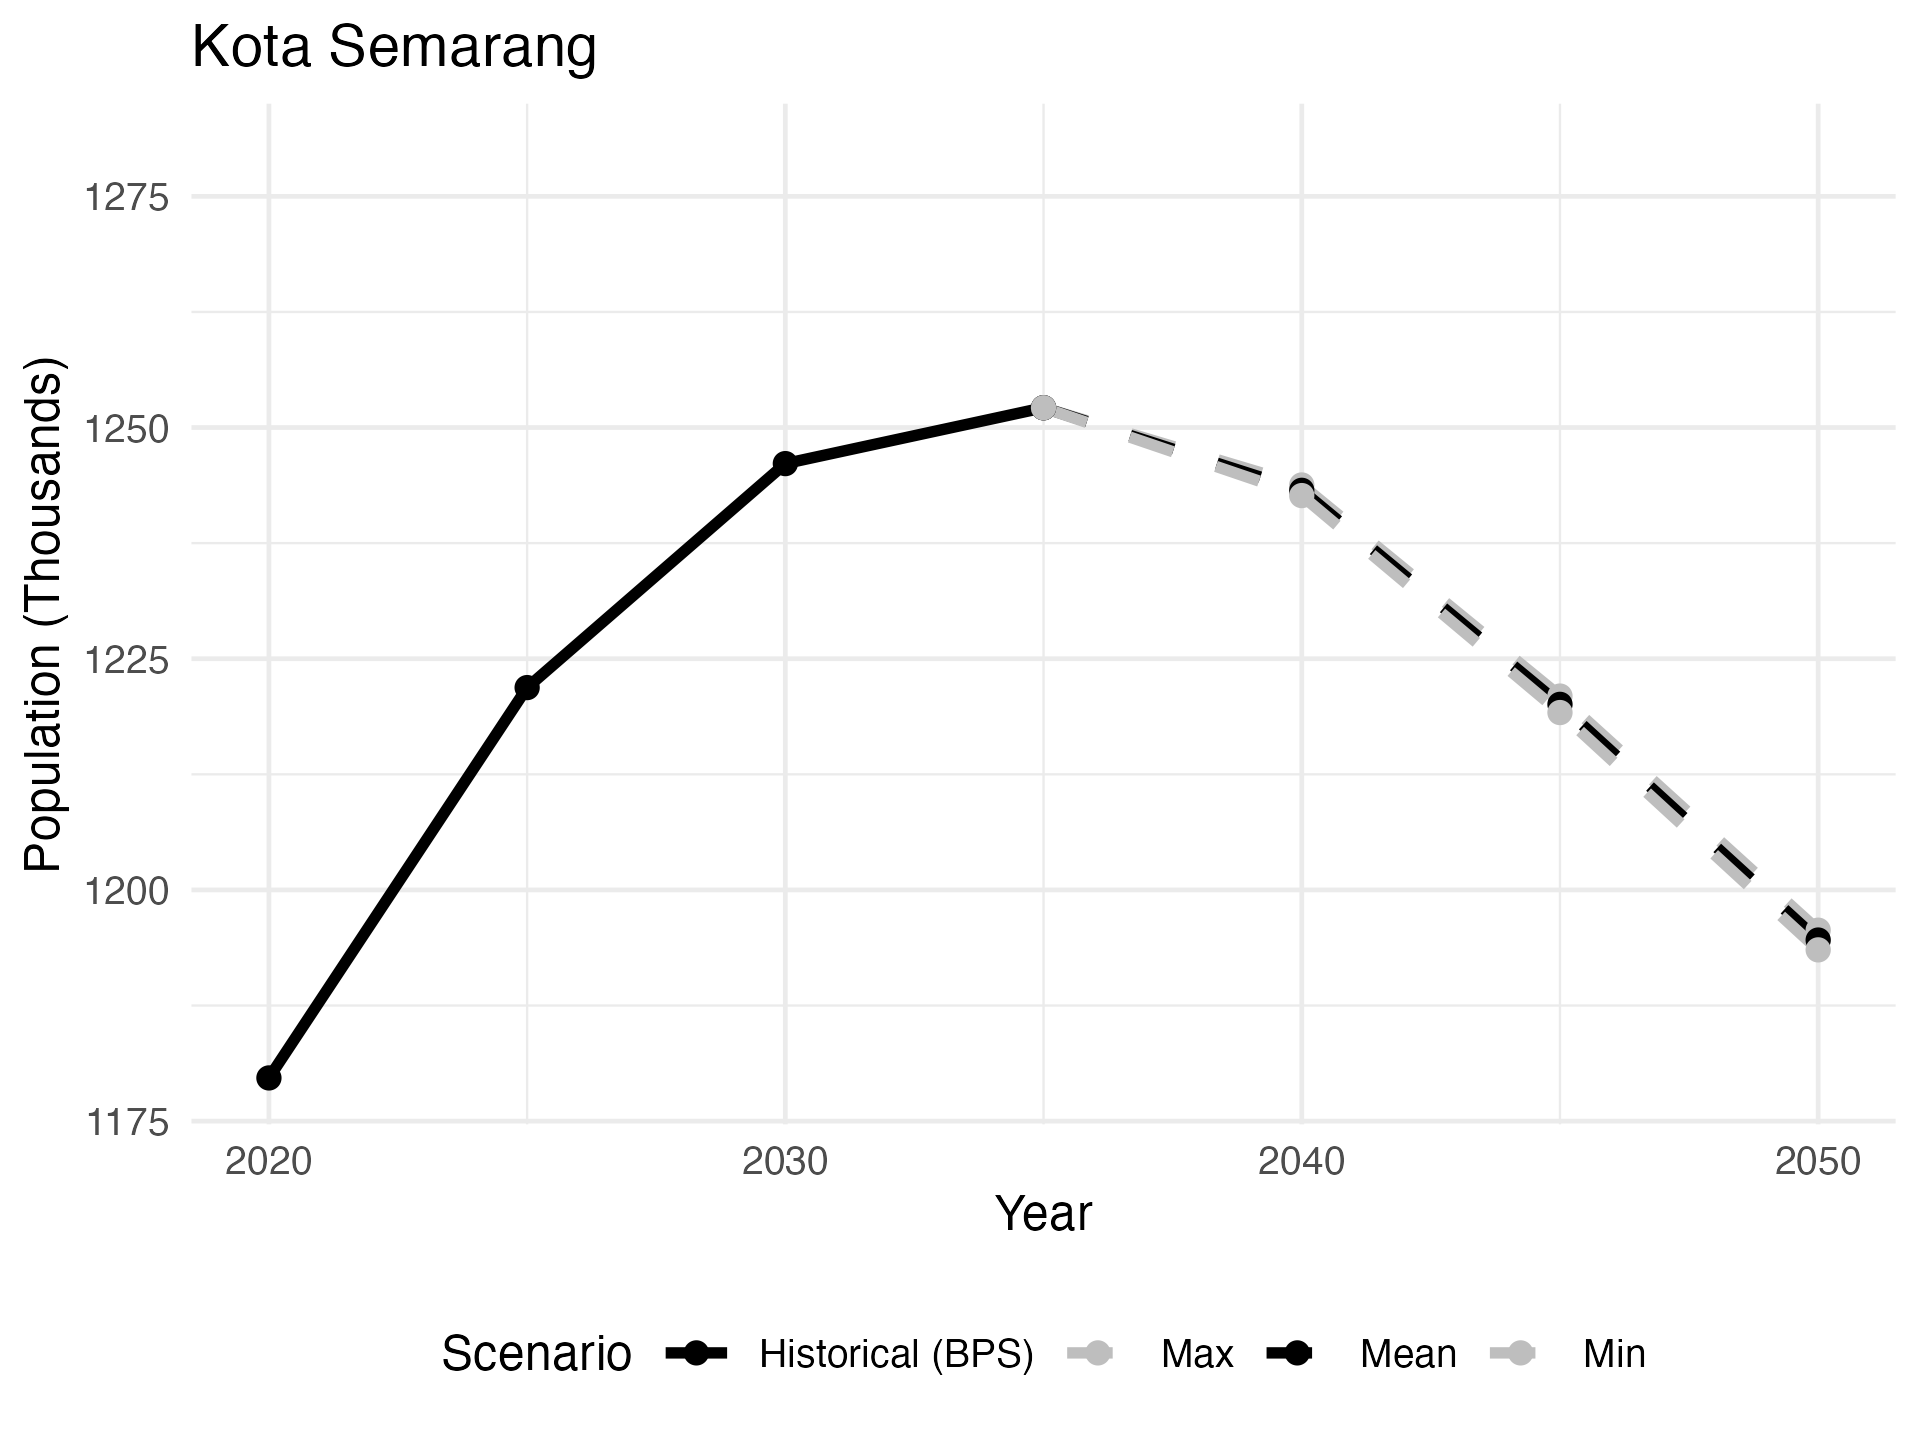
\includegraphics[width=0.5\textwidth]{img/working_kota_bw.png}
	 \caption{Working population projections for Kota Semarang}
  \label{fig:workingage_kota}
\end{figure}

\begin{figure}[htbp]
  \centering
	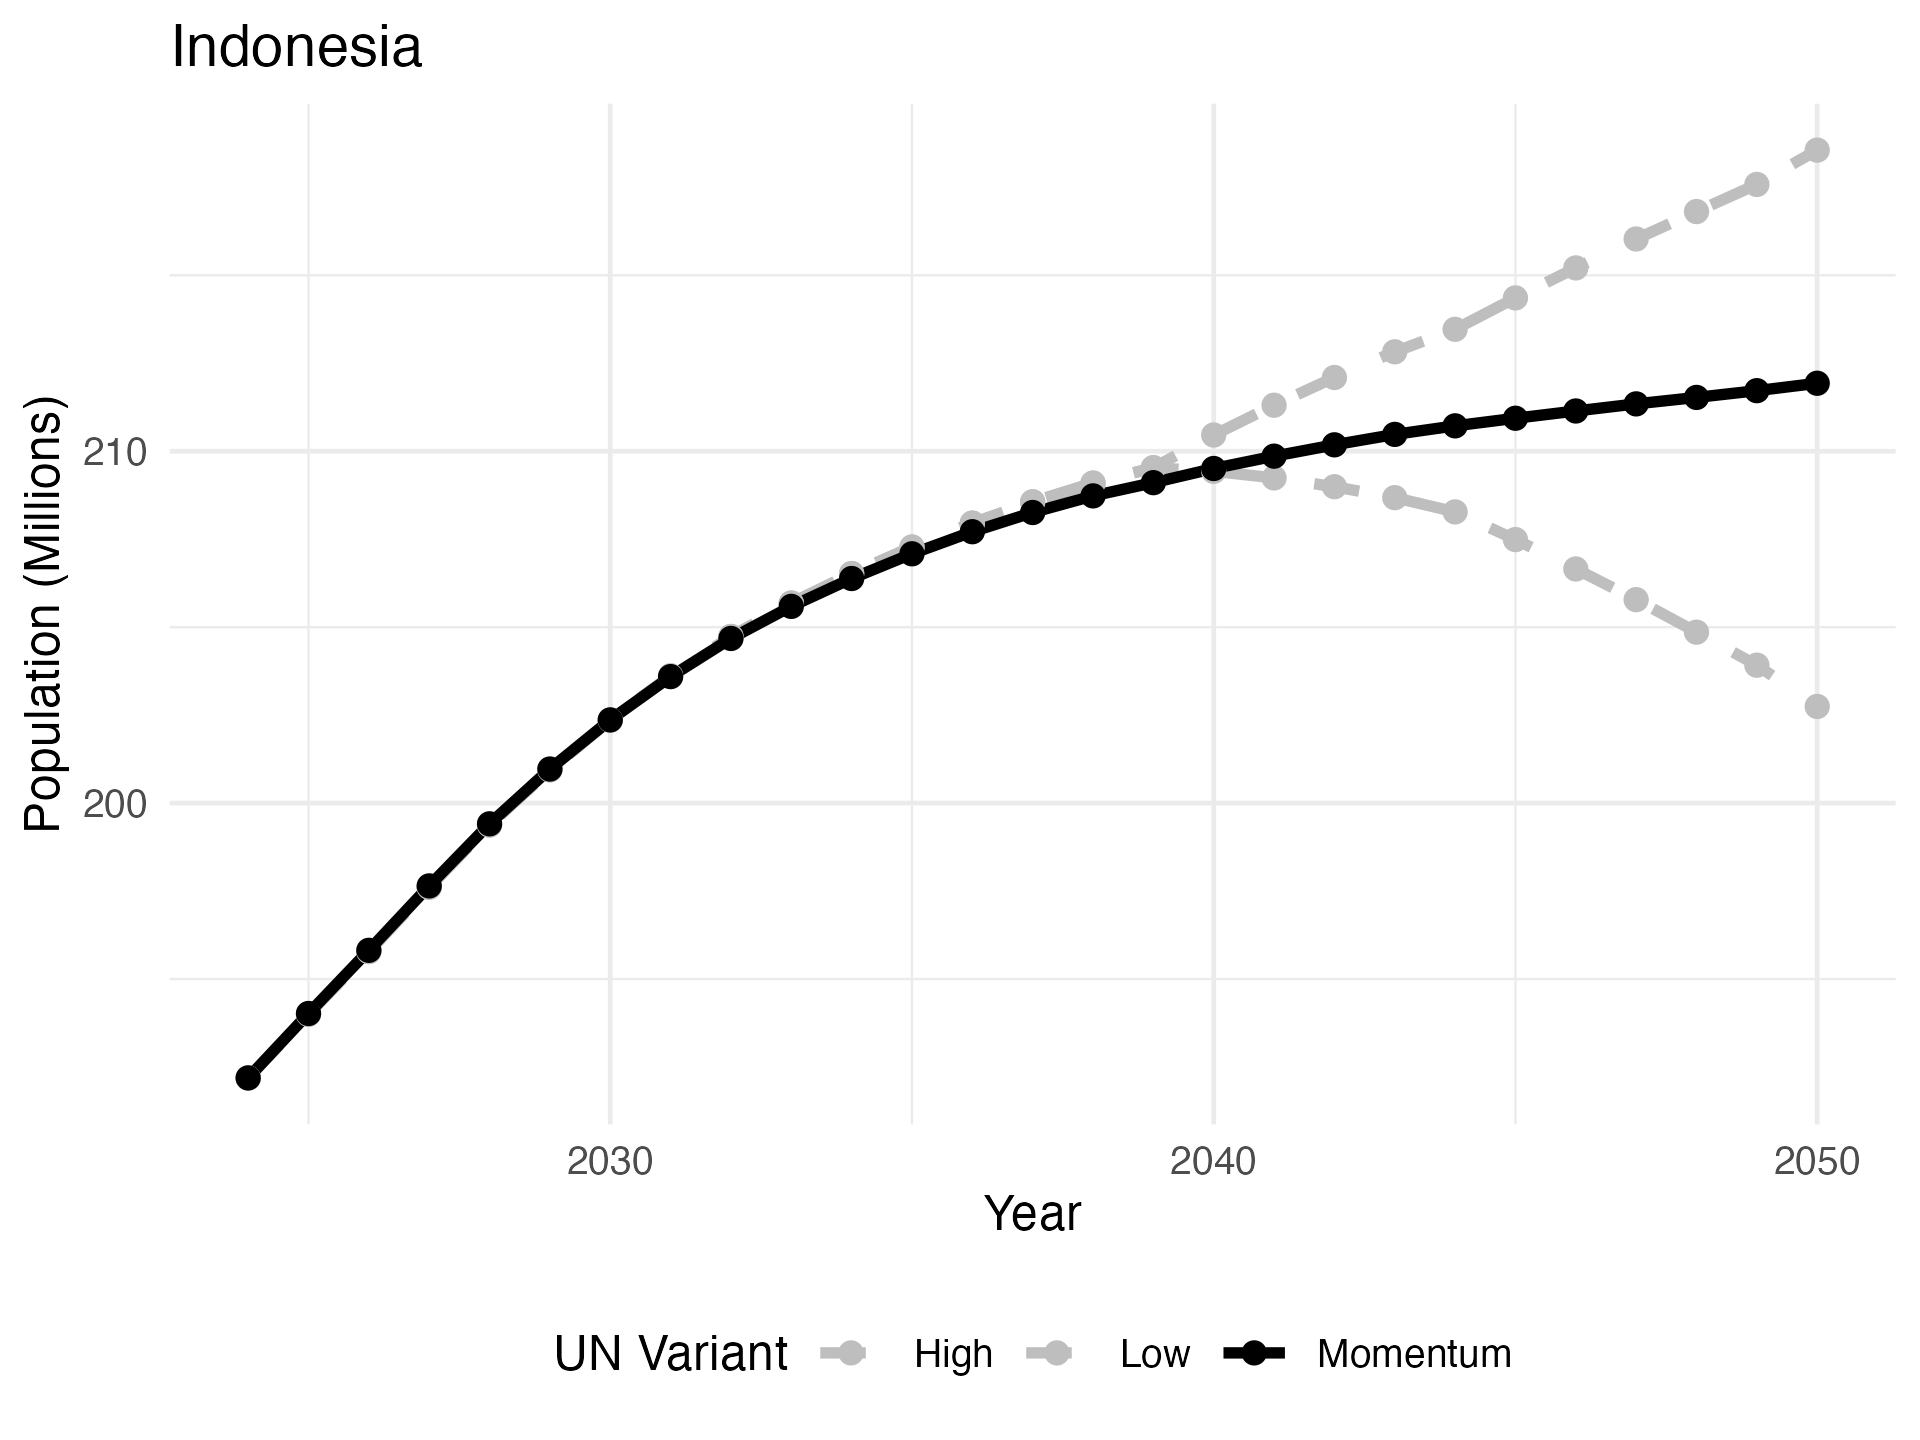
\includegraphics[width=0.5\textwidth]{img/working_country_bw.png}
	 \caption{External benchmarking comparing the projected local working-age population (ages 15-64) in Kota Semarang against the United Nations variants for Indonesia.}
  \label{fig:workingage_country}
\end{figure}

To this end, the outputs were benchmarked against the United Nations World Population Prospects (High, Low, and Momentum variants) \cite{un2024}. By executing visualizations of the projected working-age populations (ages 15--64) in Figure \ref{fig:workingage_kota} and Figure \ref{fig:workingage_country}, the model confirms that the demographic trajectory of Kota Semarang falls on the lower side within the logic and proportion when evaluated against the broader macroeconomic and demographic shifts projected for the Republic of Indonesia.

\section*{Conclusion}

The application of the Hamilton-Perry method provides a highly effective, data-efficient bridge for long-term urban forecasting. By using cohort change and child-to-woman ratios derived from limited-horizon deterministic datasets, researchers can bypass the stringent data requirements of traditional Cohort-Component Models. This framework yields plausible, scenario-bounded population matrices that enable municipal planners to prepare for future infrastructure and socioeconomic demands through 2050.

% --- BIBLIOGRAPHY ---
% Implemented natively to ensure the document remains entirely self-contained
\begin{thebibliography}{9}

\bibitem{un2024}
United Nations, Department of Economic and Social Affairs, Population Division. (2024). \textit{World Population Prospects 2024, Online Edition}. \url{https://population.un.org/}

\bibitem{bps2020}
Statistics Indonesia (BPS). \textit{Proyeksi Penduduk Kabupaten/Kota Provinsi Jawa Tengah 2020-2035 Hasil Sensus Penduduk 2020}. \url{https://jateng.bps.go.id/id/publication/2023/07/14/373be3755ab9b902b7969101/proyeksi-penduduk-kabupaten-kota-provinsi-jawa-tengah-2020-2035-hasil-sensus-penduduk-2020-.html}

\end{thebibliography}

\end{document}